\documentclass{article}
\usepackage{amsmath,amssymb, amsthm,latexsym,paralist}

\usepackage{graphicx}
\usepackage{hyperref}
\usepackage[toc,page]{appendix}
\usepackage{listings}
\usepackage{color}

\usepackage{titlesec}

\definecolor{dkgreen}{rgb}{0,0.6,0}
\definecolor{gray}{rgb}{0.5,0.5,0.5}
\definecolor{mauve}{rgb}{0.58,0,0.82}

\lstset{frame=tb,
  language=c++,
  aboveskip=3mm,
  belowskip=3mm,
  showstringspaces=false,
  columns=flexible,
  basicstyle={\small\ttfamily},
  numbers=none,
  numberstyle=\tiny\color{gray},
  keywordstyle=\color{blue},
  commentstyle=\color{dkgreen},
  stringstyle=\color{mauve},
  breaklines=true,
  breakatwhitespace=true
  tabsize=3
}

\theoremstyle{definition}
\newenvironment{problem}[1]{\noindent\textbf{Problem #1.}}{\bigbreak}
\newenvironment{solution}{\noindent\textbf{Solution.}}{\bigbreak}
\newenvironment{solutionitem}[1]{#1}{\bigbreak}

\newcommand{\name}[1]{\noindent\textbf{Name}: #1}
\newcommand{\uin}[1]{\noindent\textbf{UIN}: #1\\}

\newcommand{\problemset}[1]{\begin{center}\textbf{Homework #1}\end{center}}

\titleformat*{\section}{\bfseries}
\titleformat*{\subsection}{\large\bfseries}
\titleformat*{\subsubsection}{\large\bfseries}
\titleformat*{\paragraph}{\large\bfseries}
\titleformat*{\subparagraph}{\large\bfseries}

\begin{document}
\begin{center}
{\large
CSCE 626 - Parallel Algorithm Design and Analysis}
\end{center}
\problemset{1}

\begin{center}
\name{ Peihong Guo }
\uin{421003404}
\end{center}


\begin{problem}{1}  Given a sequence of numbers $x_1, x_2, \ldots, x_n$, the prefix sums are the partial sums
\[
\begin{split}
& s_1 = x_1 \\
& s_2 = x_1 + x_2 \\
& \ldots \\
& s_n = x_1 + x_2 + ... + x_n
\end{split}
\]
Describe an algorithm to compute the prefix sums on a PRAM with $n$
processors in $O(\log n)$ time. Analyze the running time of your
algorithm and argue, at least informally, its correctness.
Which PRAM model does your algorithm use (e.g., EREW, CREW, CRCW)?
Does your algorithm require a synchronous PRAM?
\end{problem}

\begin{solution}To obtain $O(\log n)$ running time, the computation has to be organized in a tree-like order.
  A straightforward solution is therefore compute partial sums at each step and broadcast the partial sums carefully
  to correct processors, as shown in the figure below:
  \begin{center}
    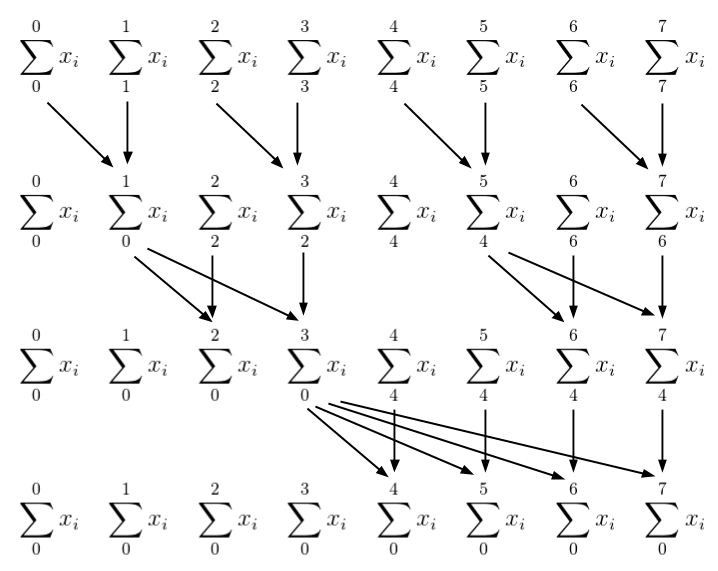
\includegraphics[width=0.65\textwidth]{naive.png}
  \end{center}
  The algorithm can be summerized by the following psedocode (suppose the ranks of the processors are from 1 to n)
  \begin{lstlisting}
    for d=1 to log2(n) do
      for all k in parallel do
        if k % 2^d == 0
          x[k] = x[k] + x[k - 2^(d-1)]
        else if k % 2^d > 2^(d-1) && k - (k%2^d) - 1 > 0
          x[k] = x[k] + x[k-(k%2^d)-1]
  \end{lstlisting}

  Clearly this algorithm has $O(\log n)$ running time because the total number of steps is $\log n$ and each step
  requires $O(1)$ time.

  We can use induction to prove the correctness of this algorithm: denote the accumulated sum at processor $j$ as $s_j$,
  then initially $s_j = x_j, j=1\ldots n$. We argue that at the $k$-th step, $s_{i2^k+1}, \ldots, s_{(i+1)2^k}$ store the
  prefix sum of elements $x_{i2^k+1}, \ldots, x_{(i+1)2^k}$, where $i = 0, 1, 2, \ldots$:
  \begin{enumerate}
  \item The argument holds after the first step because we are doing pair-wise addition every two elements.
  \item Assume after the $m$-th step, the argument holds. Then after the $(m+1)$-th step, $s_{i2^m}$ is broadcast to elements
  $s_{i2^m+1}, \ldots, s_{(i+1)2^m}$ where $i=1, 3, 5, \ldots$. Recall that $s_{i2^m+j} = \sum_{i2^m+1}^{i2^m+j}x_p$ and
  $s_{i2^m} = \sum_{(i-1)2^m+1}^{i2^m}x_p$, we have
  \[s'_{i2^m+j} = s_{i2^m+j} + s_{i2^m} = \sum_{(i-1)2^m+1}^{i2^m+j}x_p~\text{for~}j=1,2,\ldots,2^m\]
  that is:
  \[s'_{(i-1)2^m + (2^m+j)} = \sum_{(i-1)2^m+1}^{(i-1)2^m+(2^m+j)}x_p\]
  we also have
  \[s'_{(i-1)2^m + j} = \sum_{(i-1)2^m+1}^{(i-1)2^m+j}x_p\]
  where $j = 1, 2, \ldots, 2^m-1$.
  Combine the above two equations, we have
  \[s'_{(i-1)2^m + j} = \sum_{(i-1)2^m+1}^{(i-1)2^m+j}x_p\]
  where $j = 1, 2, \ldots, 2^{(m+1)}$.
  Since $i$ is an odd number, we can rewrite the above equation as
  \[s'_{\frac{i-1}{2}2^{m+1} + j} = \sum_{\frac{i-1}{2}2^{m+1}+1}^{\frac{i-1}{2}2^{m+1}+j}x_p\]
  where $j = 1, 2, \ldots, 2^{(m+1)}$. This equation has exactly the same form as our argument. Therefore the argument holds after
  the $m+1$-th step.
  \end{enumerate}
  The above analysis assumes the number of numbers equals a power of 2. For non-power-of-2 cases, the above algorithm works as well
  because we can simply ignore the broadcasting to out-of-range processors.

  The algorithm can use either of EREW, CREW and CRCW because there is no current write in the algorithm. The algorithm does not require
  a synchronous PRAM, but it does require syncrhonization at the end of each step to ensure data integrity.
\end{solution}


\begin{problem}{2} Repeat the previous question, but this time consider
  the case when $p < n$, i.e., the number of processors is less than
  the number of input elements. You should design the best algorithm
  you can in terms of time and work. Analyze the running time of your
  algorithms and argue, at least informally, their correctness.
  (If an algorithm is similar to the corresponding one from 2, you need only discuss the modifications.)
\end{problem}
\begin{solution}
  Because the number of processors $p$ is less than the number of input elements $n$, we have to perform partial computation
  and construct a final solution with the partial results.

  One way to do this is to divide the input elements into $\lceil n/p \rceil$ groups and compute prefix sum on each group using
  the parallel scan algorithm in problem 1. The groups are processed sequentially and each group would use the last sum value in
  previous group for initialization. The running time of this approach is $O(\lceil n/p \rceil \log{p})$ because each group requires $\log{p}$ time
  to process.

  Another approach is to distribute $\lceil n/p \rceil$ groups to $p$ processors and compute the prefix sum of each group locally on each
  processor. However, the sum values are not correct except for in the first group, and we need to add back the missing sum value to
  all groups but the first one. More specifically, denote the last sum value in each group as $s_i$, then value to be added back to the
  $k$-th group would be $\sum_{i=1}^{k-1}s_i$ because that is the sum of all elements preceding group $k$. Therefore, the algorithm in this
  approach can be summerized as follows (suppose $n \mod p = 0$ for simplicity):
  \begin{lstlisting}
    sz = n / p;
    for k in parallel do
      sequentially compute prefix sum for x[k*sz]...x[(k+1)*sz-1]
    s[1]...s[p] <- parallel prefix sum of (x[sz-1], x[2*sz-1], ..., x[n-1])
    for k in parallel do
      if k > 1 then add s[k] to x[k*sz]...x[(k+1)*sz-1]
  \end{lstlisting}
  The running time of this algorithm is $O(\lceil n/p \rceil + \log p)$, which is better than the first approach.

  The correctness of this algorithm is guaranteed by the correctness of sequential scan algorithm (which is trivial) and the correctness of the parallel
  scan algorithm (which is proved in problem 1), as well as the add-back step that compensate the prefix sum values exactly as needed.
\end{solution}

\flushleft\textbf{References}
\begin{enumerate}
  \item Nancy Amato. CSCE 626 Course notes.
  \item Mark Harris, Shubhabrata Sengupta and John D. Owens. Parallel Prefix Sum (Scan) with CUDA. GPU Gems 3. \\ \url{http://http.developer.nvidia.com/GPUGems3/gpugems3_ch39.html}
  \item Joseph J\'{a}l\'{a}. An introduction to parallel algorithms.
\end{enumerate}
\end{document}
